% \documentclass[lineno,twocolumn,endfloat,biblatex]{biophys-new}
\documentclass{biophys-new}
\usepackage[utf8]{inputenc}
\usepackage{graphicx}
\usepackage[colorlinks,allcolors=cyan!70!black]{hyperref}

% uncomment if using biblatex
% \addbibresource{sample.bib}

\usepackage{lipsum}
\usepackage[normalem]{ulem}

\title{Understanding the Free Energy Landscape of Phase Separation in Lipid Bilayer using Weighted Ensemble Molecular Dynamics}
\runningtitle{All plots with long captions} %% For page header

\author[1]{Ashlin Poruthoor}
\author[1,*]{Alan Grossfield}
\runningauthor{Poruthoor and Grossfield} %% For page header

\affil[1]{University of Rochester Medical Center, Rochester, NY 14620}

\corrauthor[*]{alan\_grossfield@urmc.rochester.edu}

% \papertype{Letters}
\papertype{Article}
% \papertype{Computational Tools}


\begin{document}

\begin{frontmatter}
\begin{abstract}

Lorem ipsum dolor sit amet, consectetur adipiscing elit, sed do eiusmod tempor incididunt ut labore et dolore magna aliqua. Ut enim ad minim veniam, quis nostrud exercitation ullamco laboris nisi ut aliquip ex ea commodo consequat. Duis aute irure dolor in reprehenderit in voluptate velit esse cillum dolore eu fugiat nulla pariatur. Excepteur sint occaecat cupidatat non proident, sunt in culpa qui officia deserunt mollit anim id est laborum.

\end{abstract}

\begin{sigstatement}

Lorem ipsum dolor sit amet, consectetur adipiscing elit, sed do eiusmod tempor incididunt ut labore et dolore magna aliqua. Ut enim ad minim veniam, quis nostrud exercitation ullamco laboris nisi ut aliquip ex ea commodo consequat. Duis aute irure dolor in reprehenderit in voluptate velit esse cillum dolore eu fugiat nulla pariatur. Excepteur sint occaecat cupidatat non proident, sunt in culpa qui officia deserunt mollit anim id est laborum

\end{sigstatement}

\end{frontmatter}

\section*{Introduction}

* Why phase separation is important?
* Why phase separation in cell membrane is important?
* Molecular dynamics
* Challenges of simulating phase separation using MD
* Ways to work around - CG. Enhanced sampling 
* Choice of WE

Todo list:

Figures: 

1. A figure showing individual MARTINI lipids and their AA chemDraw figure.
    A figure showing the top and side view of each lipid systems

\section*{Methods}

\subsection*{System details}

As shown in Fig 1, we used three different ternary lipid bilayer systems to test the hypothesis:
1. As the main test system, we chose a lipid bilayer consisting of dipalmitoyl-phosphatidylcholine (DPPC), dilinoleyl-phosphatidylcholine
(DIPC), and Cholesterol (CHOL) which is known to phase separate in silico in a few microseconds \cite{Risselada2008,Schafer2010,Janosi2012,Doma2012,Jong2013,Liu2020,Su2020}.
2. As a positive control, we chose a lipid bilayer consisting of DPPC, diarachidonoyl-phosphatidylcholine (DAPC), and CHOL, known to phase separate relatively faster in silico in the order of a few hundreds of nanoseconds \cite{Lin2016,Lin2019,Davis2013a}.
3. As a negative control, we chose a lipid bilayer consisting of DPPC, palmitoyl-oleoyl-phosphatidylcholine (POPC), and CHOL that was previously shown not to
phase separate \cite{Veatch2003,Davis2013a}.
The composition of DPPC-DIPC-CHOL, DPPC-DAPC-CHOL, and DPPC-POPC-CHOL systems used here are (0.42/0.28/0.3),
(0.5/0.3/0.2) and (0.4/0.4/0.2) respectively and were adapted from previous studies \cite{Risselada2008,Lin2016,Davis2013a}.

Due to the relatively larger system size and time scale required for phase separation and related dynamics in lipid bilayer simulations, the Coarse-Grained (CG) model of 
each system was used.
Hence the subsequent dynamics propagation using MD is relatively cheaper than an All-Atom model but with the tradeoff in system resolution.
The rationale behind this design choice is to fail faster with minimum resources if this proof-of-concept protocol is not working as expected. 
Using CHARMM-GUI Martini Maker \cite{Qi2015}, we constructed four random replicas of each CG ternary symmetric bilayer system.
MARTINI 2 force field parameters and particle definitions\cite{Marrink2007,DeJong2013} were used to construct CG systems and to run the subsequent MD simulation. 
The default input files from CHARMM-GUI Martini Maker were replaced with their respective most recent Martini 2.x versions, if they existed.
MARTINI polarizable water model\cite{Yesylevskyy2010} was used to solvate all systems with approximately a 1:30 lipid to real water ratio.
A detailed description of the systems used can be found in the Table S1 of supplementary material.

\subsection*{Standard MD simulation details}

Due to the historical compatibility of the the GROMACS MD engine with the MARTINI force field, we used GROMACS 2020.3\cite{Abraham2015} to propagate the dynamics of the systems prepared. 
Each system was minimized and equilibrated in steps using the MD input files suggested by CHARMM-GUI Martini Maker.
To obtain an intact bilayer without any membrane undulations, we used an additional membrane restraining protocol: 
We took advantage of the flat bottom restrain potential available in GROMACS to allow lipids to move freely in the $xy$ plane but restrained within a slab of
defined z thickness.
More details about membrane restraining protocol can be found in the supplementary material.

After the minimization and equilibration, all systems were run at 400 K in the NPT ensemble for 100 ns to make sure the lipids in each system were
randomly distributed.
For every system, each replica was then forked into multiple temperature runs simulated at different temperatures ranging from 298K to 450K. 
%\sout{For every system, each replica was then forked into multiple temperature runs. 
%For the positive control, DPPC-DAPC-CHOL lipid bilayer system, every replica was simulated at 298 K, 323 K, 333 K, 343 K, 353 K, 373 K, 423 K and, 450 K. 
%For the main test system, DPPC-DIPC-CHOL lipid bilayer, every replica was simulated at 298 K, 323 K, 333 K, 343 K, 353 K, 423 K, and 450 K. 
%For the negative control, DPPC-POPC-CHOL lipid bilayer system, every replica was simulated at 298 K, 323 K, and 450 K.}
All standard MD simulations were run for at least 8 microseconds using the BlueHive supercomputing cluster of the Center for Integrated Research and
Computing at the University of Rochester. Simulations were run on Intel Xeon E5-2695 and Gold 6130 processors augmented with Tesla K20Xm, K80, and V100 GPUs.   
The trajectories were processed and analyzed using LOOS software package.
A detailed description of the simulation parameters can be found in the Table S1 of supplementary material.  

\subsection*{Collective Variable}

A collective variable (or a set of variables) is a reduced coordinate that captures the progress of a system along the transition of interest.
Ideally, such a reduced variable(s) should fully capture the key modes of transition to reflect the complex event under study.
The success of any enhanced sampling protocol depends on the chosen collective variable over which the sampling is enhanced\cite{Valsson2016,Yang2019b,Henin2022}. 
In our case, phase separation in a  quantifies the recruitment of lipids into such domains could be used to track the phase separation
events in our systems. Here, we define lipid bilayer is characterized by the formation of lipid domains with distinct properties from the rest of the bilayer.
Hence we hypothesized that a variable thatthe Fraction of Lipids in Cluster (FLC) as follows:

\begin{equation}
\label{eq:CLT}
\text{FLC} = \sum_{i}^{N} \frac{\text{No. of $X_i$ lipids in lipid $X_i$ Clusters}}{\text{No. of Lipid $X_i$}} =  \frac{\sum_{i}^{N} \text{No. of Lipid X$_i$ in Lipid X$_i$ Clusters}}{\text{Total No. of Lipids}}
\end{equation}


Where subscript $i$ denotes the individual lipid species in a bilayer consisting of N total lipid species.
As shown in Figure 2, each system has $N=3$ lipid species in our case.
FLC increases as the system go from a mixed state, with a random distribution of lipids, to a separated state.
In principle, FLC is bounded between 0 and 1. FLC = 0 corresponds to a system configuration where no lipids are part of any cluster.
While FLC = 1 corresponds to all lipids being a part of some cluster. 

%\ref{fig2:view}
\begin{figure}[hbt!]
\centering
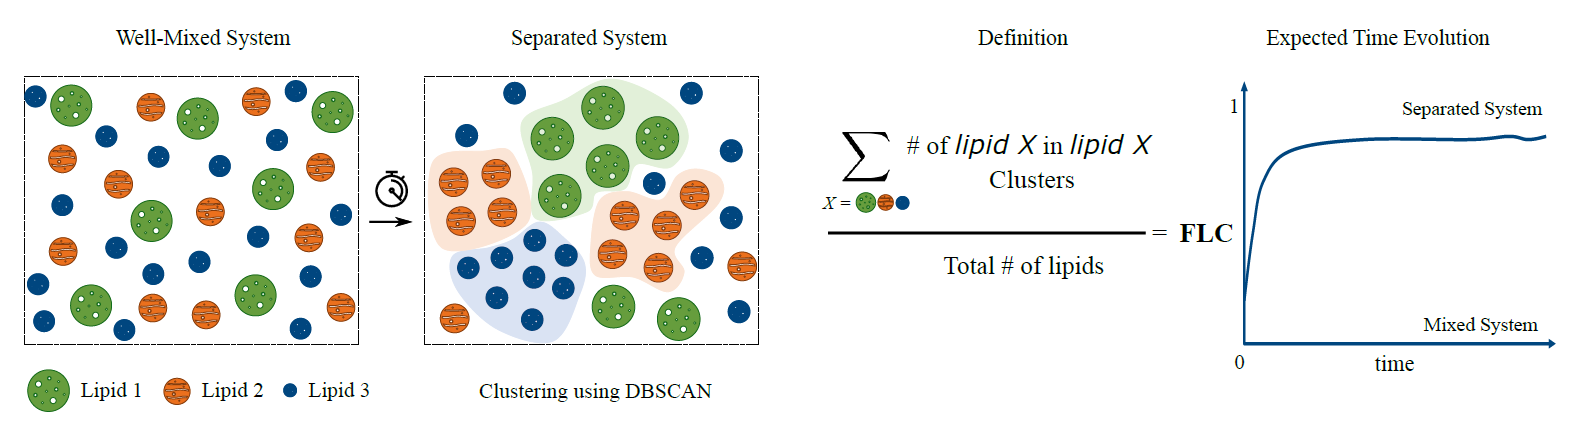
\includegraphics[width=1\linewidth]{Figures/Figure1.PNG}
\caption{a. A phase separating system evolves from a mixed state to a separated state. b. Functional form of FLC. c. FLC evolution curve for a phase separating system}
\label{fig2:view}

\end{figure}


The lipid $X_i$ cluster is defined using the Density-Based Spatial Clustering of Applications with Noise (DBSCAN) algorithm \cite{MartinEsterHans-PeterKriegelJiirgSander1996,Ester2017} as implemented in scikit-learn \cite{PedregosaF.VaroquauxG.GramfortA.MichelV.ThirionB.GriselO.BlondelM.PrettenhoferP.WeissR.andDubourgV.VanderplasJ.PassosA.CournapeauD.BrucherM.PerrotM.Duchesnay2011}.
For lipid DBSCAN clustering, instead of the default euclidean metric to calculate the distance between lipid coordinates, we used a precomputed distance matrix adjusted for periodic boundary conditions of the simulation box using LOOS.
Two additional input parameters are required by the algorithm: $min\_samples$ and $\varepsilon$.
Lipids with more than $min\_samples$ neighbors (including the lipid itself) within $\varepsilon$ radius are considered as core lipids.
Non-core lipids that are still within $\varepsilon$ radius of a core lipid are considered border lipids.
A set of core lipids within $\varepsilon$ radius of each other and their border lipids forms a cluster.
All lipids that are not a part of any cluster are considered outlier lipids.

Since lipid motion in a bilayer is mostly constrained in a plane and MARTINI beads for a lipid are of similar radii, we can make use of the two-dimensional
version of Kepler's conjecture that the densest packing of unit disks in a plane is hexagonal close packing (Thue's Theorem).
Hence we chose 7 (6 nearest neighbors + 1 central lipid) as $min\_samples$ for all the lipid species.
However, $\varepsilon$ was chosen differently for each lipid species based on their first nearest neighbor distance from the central lipid.
The first nearest neighbor distance of an individual lipid species was calculated using the $xy\_rdf$ tool in LOOS.
From the first 8 $\mu$s MD standard simulation of each replica, we computed the radial distribution function (RDF) for a lipid species in the xy-plane. 
From the RDF plot, we found the first maxima (provided it is above 1), and the distance to the minima right after this first maxima were determined to be the first nearest neighbor distance for that lipid species.
This distance was averaged over all four replicas for a given system at a given temperature and was assigned as the respective $\varepsilon$ input.
Since nearest neighbor distance is a function of temperature, for the same lipid species in the same system, $\varepsilon$ may be different for different temperatures.
Computed $\varepsilon$, i.e., average first nearest neighbor distance for different conditions are plotted in Supplementary Figure S1.

\subsection*{Auxiliary Variables}

Additional auxiliary variables (AVs) were tracked parallel to the primary collective variable, FLC. 
Following are the definitions of AVs that evaluate the quality of DBSCAN clustering since it is critical for defining the FLC that drives the WE equilibrium dynamics. 
For each lipid species, $X$ in the system, we calculated the following, 

1. Number of $X$ clusters in the system under study.

2. Fraction of $X_i$ lipids in $X$ clusters

3. Fraction of $X_i$ lipids in $X$ core lipids.

4. Mean Silhouette Coefficient (MSC) of $X_i$ Clusters, as implemented in scikit-learn.

Silhouette Coefficient is a method used to evaluate the clustering done by any technique, especially if ground truth labels are unknown. 
Here, for a $X_i$ lipid in the cluster, mean intra-cluster distance (a) from other $X_i$ lipids in the cluster is found.  
Similarly, for a $X_i$ lipid in the cluster, the mean nearest-cluster distance (b) is also calculated.
While the former assesses the 'cohesion' of a given $X_i$ lipids with other $X_1$ lipids in a cluster, the latter assesses the 'separation' from the nearest cluster.
Thus, Silhouette Coefficient for a $X_i$ lipid, s, is defined as below,

\begin{equation}
\label{eq:SC}
\text{s} = \frac{b - a}{max(a,b)}
\end{equation}

The Mean Silhouette Coefficient of $X_i$ Clusters is given by the mean $s$ over all non-outlier $X_i$ lipids.
Here, we have omitted the MSC calculations for cases when there are no clusters or just one cluster detected by DBSCAN. 
MSC is bound between and -1 and 1.
A high positive value corresponds to well segregated dense clusters, while a low negative value implies that lipids are assigned to clusters incorrectly.  

Similar to the FLC, a set of additional AVs that track phase separation are also defined as given below.
The rationale behind such AVs is to serve as proxy coordinates that can independently assess phase separation events enhanced by FLC driven WE runs.
\\

1. Cumulative Enrichment Index (CEI): 

We defined a density based quantity to estimate the degree of global lipid enrichment in the system, similar to the ones that track local lipid segregation used previously \cite{Gu2019, Gu2020}.
Here, we calculated the average local density of $X_i$ lipids around a single lipid $X_{ij}$, within a cutoff radius, $\epsilon_i$, as we defined earlier for FLC estimation.
The cutoff radius, $\epsilon_i$, is also temperature dependent.
We also defined a normalization factor, $\Phi_i$, as the local density of $X_i$ lipids for a uniformly well mixed system of similar composition.
The ratio of former respective to latter forms the enrichment index for a lipid species, $X_i$ .
CEI is defined as the sum of individual enrichment index for all the lipid species in the system, as follows:  

\begin{equation}
    \begin{aligned}
    \label{eq:CLT}
    \text{CEI} {}   & = \sum_{i}^{N}\Bigg[\frac{\text{Average local density of lipids $X_i$ around a single lipid $X_i$}}{\text{Local density of lipid $X_i$ for a well mixed system}}\Bigg]_{\text{$\epsilon_i(T)$}} \\
                    & =  \sum_{i}^{N} \frac{1}{\Phi_i}\frac{1}{\text{$\pi\epsilon_i^2$}}\sum_{j}\text{No. of $X_i$ lipids around $X_{ij}$ lipid in $\epsilon_i(T)$ radius}
    \end{aligned}
\end{equation}

Where $X_{ij}$ denotes $j^{th}$ lipid of $X_i$ lipid species.
The local density around $X_{ij}$ is calculated within $\epsilon_i(T)$ distance, where T is the temperature of the system.
We do correct the local density for central lipid contributions.
For the normalization factor, $\Phi_i$ the global density of $X_i$ lipids is calculated by taking the ratio of total number of $X_i$ lipids in the system to the $xy$-planar area of the bilayer system.
For a uniformly well-mixed system, this global density is same as local density of $X_{i}$ lipid.
Thus CEI $>$ 3 implies that the ternary system, $N=3$, is deviating from well mixed state to more separated state. 
\\

2. Segregation Index (SI)

We defined a contact based quantity to track the homogenity of lipid bilayer, similar to the ones that track mixing of beads used previously\cite{Marigo2012,Kumar2020}.
Here, we calculated the fraction of like contacts made between $X_i$ species with respect to the total contacts made by $X_i$ as shown below:

\begin{equation}
    \begin{aligned}
    \label{eq:CLT}
    \text{SI} = \sum_{i}^{N}\Bigg[\frac{X_iX_i}{\sum_{j}^{N}X_iX_j}\Bigg]_{\text{$\epsilon_i(T)$}} = \frac{X_{11}}{X_{11} + X_{12} + X_{13}} + \frac{X_{22}}{X_{21} + X_{22} + X_{23}} + \frac{X_{33}}{X_{31} + X_{32} + X_{33}}
    \end{aligned}
\end{equation}

Where $X_iX_j$ denotes the contacts made between lipid species $X_i$ and $X_j$ within $\epsilon_i(T)$ cutoff.
Thus for a ternary bilayer system, SI $=$ 3 implies a fully separated system and SI $<$ 3 implies mixing.
However, for the analysis here, we ignored the contribution of Cholesterol as we found that excluding Cholesterol term did not change the functional behavior (Supplementary Info).
Hence, $\text{SI}_{\text{noCHOL}}$ effectively will have bounds [0, 2] unless otherwise stated.    

\subsection*{Weighted Ensemble Simulation}

\textbf{Preparing seeding configurations for WE simulation:} 
From each 8 $\mu$s replica MD simulation of a given system, the last 10 frames spaced by 100 ns were collected.
Using such collected frames, we created sets of mixed and separated configurations for each replica of a given system.
For DPPC-DAPC-CHOL and DPPC-DIPC-CHOL systems, the set of mixed configurations for a particular replica came from the respective 423 K and 450 K simulation frames. 
While the set of separated configurations for a replica came from  the respective 298K and 323K simulation frames.
For the DPPC-POPC-CHOL system, sets of mixed and separated configurations for a replica came from the 450 K and 298K simulation frames respectively.
To enhance the convergence of WE equilibrium simulations, we decided to seed each simulation from both mixed and separated states and let the enhanced sampling cover the transition between them.

\textbf{Running WE simulations:} 
Weighted Ensemble equilibrium simulations were run using the WESTPA 1.0 software package\cite{Zwier2015} following the previosly established protocol\cite{Bogetti2019}.
The collective variable was divided into 30 dynamic bins using the minimal adaptive binning scheme (MAB)\cite{Torrillo2021}.
For each replica, a target number of 4 short simulations, or "walkers" per bin, were started in parallel from the mixed and the separated configurations prepared earlier.
After every resampling interval of 1 ns, the collective variable was evaluated to initiate the merging and splitting of walkers to maintain the target number of walkers per bin.
A short 1 ns MD run of all the walkers and subsequent resampling, according to the standard WE algorithm, constituted 1 WE iteration. 
We conducted 500 WE iterations for each replica.
The MD propagation was done using GROMACS 2020.3 engine with the same parameters used for standard MD simulations described earlier.
A WE Equilibrium Dynamics (WEED) reweighting protocol\cite{Bhatt2010,Suarez2014}, implemented in WESTPA 1.0, was used to accelerate the convergence of WE walkers into an equilibrium. 
The reweighting was done every 10 WE iterations.
For the DPPC-DAPC-CHOL, DPPC-DIPC-CHOL, and DPPC-POPC-CHOL lipid bilayer systems, four WE replicas were simulated each at multiple temperatures. 
All WE runs were carried out using the Intel Xeon E5-2695 and Tesla K20Xm GPUs in the BlueHive supercomputing cluster of the Center for Integrated Research and
Computing at the University of Rochester.   

\textbf{Analysis of WE simulations:}
The probability distribution of CV and AVs for each replica, as a function of WE iterations, was constructed using $w\_pdist$ and $plothist$ tools in WESTPA.
Using this distribution, we monitored the evolution of each WE replica simulation and the convergence.
$w\_mult\_west$ tool in WESTPA was used to combine data from four WE replicas of a system at a given temperature.
From the combined probability distribution of a system, the respective Free Energy Surface (FES) was created.
To check the flux between states and population in different states, $w\_ipa$, another WESTPA tool, was used.

\section*{Results}

Consistant with previous studies from which they are adapted, the standard CG MD simulations of DPPC-(DA/DI)PC-CHOL systems phase separates into $\text{L}_{\text{o}}$ and $\text{L}_{\text{d}}$ regions.
$\text{L}_{\text{o}}$ region enriched in saturated lipid, DPPC, and Cholesterol. 
$\text{L}_{\text{d}}$ region is enriched with unsaturated lipids (DA/DI)PC.
The DPPC-POPC-CHOL system showed low to no separation.
In this section, we first compare how different variables track phase separation propensity in lipid bilayers using standard CG MD simulations.
We then compare the convergence of WE simulation with respect to choice of collective variable.
Finally, we present the free energy landscapes of lipid bilayer systems obtained using WE simulations and discuss about reusing the data generated to form further intutions and applications.

\subsection*{Tracking phase separating lipid bilayers}

To evaluate how collective variable, FLC, and other auxillary variables track phase separation in lipid bilayers,
from standard CG MD, we traced the time evolution of each variable for different systems at different temperatures.
The Figure 3 illustrates the temporal evolution of FLC, CEI and $\text{SI}_{\text{noCHOL}}$ for DPPC-(DA/DI/PO)PC-CHOL systems at 298K, 323K, 423K and 450K.
For DPPC-(DA/DI)PC-CHOL systems, the variables capture a single transition between a mixed state and a separated state.
Also, the sytems reside dominantly in separated state after the transition in the standard CG simulation.
Interestingly, for relatively slow separating DPPC-DIPC-CHOL, CEI and $\text{SI}_{\text{noCHOL}}$ tracks a relatively slower state transition than FLC.
However, for DPPC-POPC-CHOL system, the variables capture a single state corresponnding to a mixed system and no transition.
But it is worthy to note that FLC, CEI and $\text{SI}_{\text{noCHOL}}$ captures the effect of temperature in all systems, including the negative control that does not phase separate.
These variables even captures the subtle differences in phase separating propensity between systems.
For example, at 298K, the plateaued region of the FLC, CEI and $\text{SI}_{\text{noCHOL}}$ curves are higher for DPPC-DAPC-CHOL system than the DPPC-DIPC-CHOL system.
This is expected as (a) the lipid chain mismatch between saturated and unsaturated lipid species and (b) the number of double bonds in unsaturated lipid species is more in the DPPC-DAPC-CHOL than DPPC-DIPC-CHOL system.
Both these factors have previously shown to influence lipid phase separation kinetics and domain stablity\cite{Fowler2016,Lin2016}.
Thus we have a set of low-dimensional variables that can (a) represent the global dynamics of the lipid bilayer system,
(b) distinguish and track the transition between mixed and separated states, (c) capture the temperature effects,
and (d) based on the compostion of the system.
The time evolution of other auxillary variables can be found in Fig SX.
\\

\subsection*{Choice of collective variables for WE simulations}

Since the density based, CEI, contact based $\text{SI}_{\text{noCHOL}}$ and clustering based FLC tracks bilayer lipid separation simliarly,
we decided to use them as progress coordinates to drive the WE simulation.
However, the free energy landscapes generated, using these variables, after running 500 WE iterations give conflicting results for the same system.
As shown in Figure 4A, for the test system DPPC-DIPC-CHOL replica at 323K, free energy landscape do not agree with each other despite the number of WE iterations used to construct them are same.
From CEI free energy landscape, we see both states are equally likely.
$\text{SI}_{\text{noCHOL}}$ landscape suggests mixed state is more likely than the separated state.
However, both these results deviate from what we observe with standard CG MD simulation,
where the DPPC-DIPC-CHOL system slowly separates into $\text{L}_{\text{d}}$ and $\text{L}_{\text{o}}$ regions and stay separated for the most of simulation.
Moreover, disagreement of free energy curves as a function of WE iteration blocks used to generate them, suggest that the underlying sampling has not converged enough.
On the other hand, FLC free energy landscape shows separated state is favorable but the free energy barrier between the two states is small.
Additionally, there is a convergence between FLC free energy curves as we proceed with WE iterations.
Thus, all three free energy landscapes show a double-well, identifying two states but disagree on the state the system is most likely to be in, and the relative free energy difference between states.
Interestingly, if we monitor the evolution of configurational distributions of each variable, as a function of WE iterations, all three show a converged behavior as shown in Fig 4B.

These conflicting results raise the following questions: Why does variables that make perfect sense while tracking the system in standard CG MD simulation, gives differnet free energy landscape after WE simualtion?
Why does CEI and $\text{SI}_{\text{noCHOL}}$ that show converged configurational distributions as a function of WE iterations, does not give converged free energy curves with each other as WE proceeds?

The configurational distribution of collective variables staying mostly undisturbed in two states (Fig 4B) and
the free energy curves struggling to converge on the state basins and free energy barrier for CEI and $\text{SI}_{\text{noCHOL}}$ landscapes (Fig 4C) 
suggest  that there might not be adequate state crossing of walkers populating each state.
Hence we decided to check the flow rate of probability across the states.
To calculate the flux between states, we need to define the states for each collective variable.
We define mixed and separated states as CEI = [0.0, 3.9] and [4.4, 6.0], $\text{SI}_{\text{noCHOL}}$ = [0.0, 1.3] and [1.4, 2.0], and FLC = [0.0, 0.575] and [0.65, 1.0] repectively.
Please note that the state bounds are chosen based on visual inspection of the corresponding free energy landscapes given in Fig 4A.
The choice is arbitary but ad hoc enough to give us a picture of what's happening. 
Fig 4C shows the mean flux from mixed to separated state and vice versa in WE simulation driven using each collective variable.
Here, mean flux is calculated for a window of 10 WE iterations as the WEED reweighting protocol is done every 10 iterations to accelerate the convergence.
The peaks in these plots implies probability crossing states.
For CEI, no state crossing occurs between mixed to demixed, and vice versa during WE simulation.
For $\text{SI}_{\text{noCHOL}}$, the state crossing back and forth is practicaly zero during first few hundreds of WE iterations.
Meanwhile for FLC, flux into and out of the states is relatively higher and immediate than other two variables.
These results are supported by the corresponding state population evolution as a fucntion of WE iterations as shown in Fig 4D.
Here, normalized walker population occupying a specific state is calculated for a window of 10 WE iterations simialr to Fig 4C.

The walkers crossing bins and thereby constituting a flow of probability between states is crucial for the success of a WE equilibrium simulation\cite{Zuckerman2017}.
Thus these results suggests that for CEI and $\text{SI}_{\text{noCHOL}}$ variables, the initial distribution of walkers is not disturbed throughout the WE simulation.
Without sufficent state crossing, the initial configurational distribution is not relaxing into a well sampled equilibrium distribution for WE simulations driven by CEI and $\text{SI}_{\text{noCHOL}}$ even after 500 iterations. 
This explains why in free energy landscapes associated with CEI and $\text{SI}_{\text{noCHOL}}$, we do not see converged free energy curves as WE proceed.
But for FLC, we see sufficent state crossing and a relatively well converged free energy curves as WE proceeds. 
The combined results from standard CG MD and WE simulations suggests that CEI and $\text{SI}_{\text{noCHOL}}$ are good proxy labels for phase separation but poor choice for collective variable to drive WE simulations.
Additionally, we found that free energy curves generated by FLC driven WE simulation are consistant across replicates as well (Fig SX).
Hence we decide to go forward with FLC based WE simulation to enhance the sampling of phase separation events in lipid bilayer systems to understand the underlying thermodynamics.
\\ 
\subsection*{Free energy landscapes of lipid bilayer systems}

Figure 5 shows the free energy profiles of DPPC-DAPC-CHOL, DPPC-DIPC-CHOL and DPPC-POPC-CHOL lipid bilayer systems.
Each curve is generated by averaging four WE replica simulations as mentioned in Methods section.
Individual replica contribution is obtained by averaging last 10 iterations of the respective replica WE simulation (491-500). 
The positive control, DPPC-DAPC-CHOL system that readily phase separates has a double well behavior at 323K and 353K.
However, both basins corresponds to relatively high FLC.
In addition to the free energy curve at 423 K, we see that regardless of high temperature this system prefers to be in configurations where more than 60\% of lipids are in some clusters.
For the negative control, DPPC-POPC-CHOL system, the free energy curves at 298K and 423K have single well nature and correpsonds to low fraction of lipids prefering to be in any clusters.
For the test system, DPPC-DIPC-CHOL system, as the temperature increases, the characteristic double well, transition to single well curves and the width of free energy curves decreases.
In general, FLC based free energy landscapes captures the role of lipid species constituting the bilayer system in its phase separation.
Moreover, the effect of temperature in decreasing the propensity of a lipid bilayer to separate is evident in all system.
It should be noted that, though the expectation of clustering based FLC is to track formation of domains in lipid bilayer, the fact that it also neatly captures the temperature effect even for the negative control, suggests the robustness of FLC as collective variable.

\subsection*{Reusing simulation data}

One of the outcome of WE simulation is the curated ensemble of diverse trajectories/walkers.
By construction, WE resampling ensures the weights associated with these walkers are unbiased.
Thus, we can reuse these weights to examine other variables of choice post-simulation.
Assuming the initial configurational distribution relaxed into an equilibrium distribution during WE simulation driven by FLC (see Discussion), 
reusing the weights, here we have reconstructed anologous free energy landscapes with other variables.

provided there's an equilibrium distribution are can be reused


weights to indicate the relative importance of any given region at any time


%\subsubsection*{Rescuing poor performing collective variables}

%\subsubsection*{$\Delta\Delta$G profile}


\section*{Discussion}

1. Outline the FLOPSS pipeline (Take that damn figure from student seminar slides to avoid writing a ton of stuff)

2. What we achieved

3. Where we are going with this




% ------------------------- %
% Uncomment if using bibtex (default)
\bibliography{PhaseSeparationArticle}

\end{document}